链队有队空的情况:L-\textgreater{}rear==NULL或者L-\textgreater{}front==
NULL。

可以这样记住,因为只要链队为非空,二者值都不应该为NULL,反之为空。

链队在内存无限制的情况下,无队满的情况。

\textbf{1. 进队(类似在链表尾进行插入操作)}

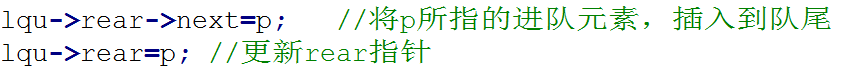
\includegraphics[width=3.59375in,height=0.29167in]{png-jpeg-pics/3206F0D598775FA50B01A619C98149DD.png}

\textbf{2. 出队(类似在链表头进行删除操作)}

\textbf{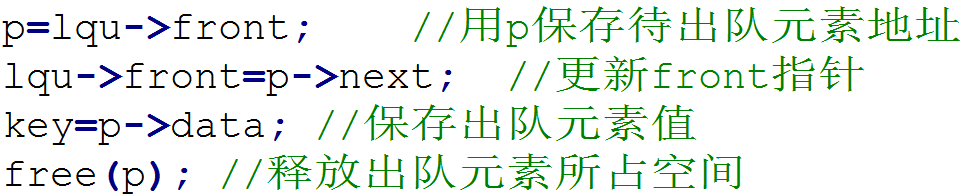
\includegraphics[width=2.91667in,height=0.59375in]{png-jpeg-pics/09CCBBEDE3B087877C02A1E27C117DF0.png}\\
}
